\documentclass{article} \usepackage{pgfplots}
\usepackage{tikz}
\usepackage{amsmath}
\usepgfplotslibrary{fillbetween}
\pgfplotsset{compat=1.15}

\title{ AP Calculus AB Take-Home Final }
\begin{document}
\author{
	Duncan Freeman
}

\maketitle

% Also make boxing answers a thing ala https://tex.stackexchange.com/questions/20575/attractive-boxed-equations#20582
% Finally, add 'k' and 'j' labels to the graph on problem 1
% Convert to a function for Problem 4

\pagebreak
\section{}
\begin{center}
	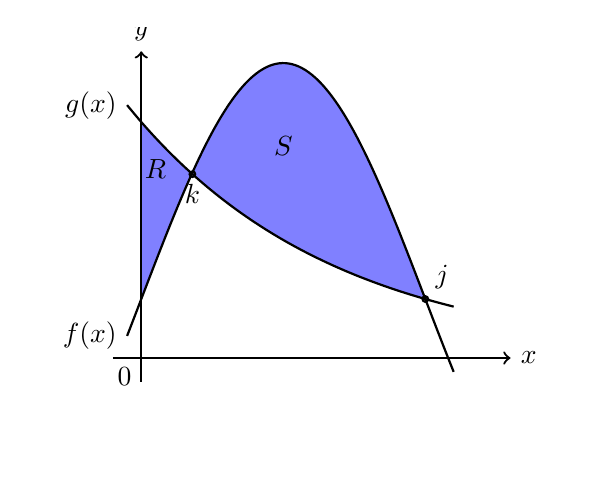
\begin{tikzpicture}
		\begin{axis}[thick,smooth,no markers, hide axis, ymin=-0.5, ymax=1.4, xmin=-0.4, xmax=1.5]
			\addplot+[name path=A,black, samples=100, domain=-0.05:1.1] {0.25 + sin((\x * pi) r)} node[left, pos=0] {$f(x)$};
			\addplot+[name path=B,black, domain=-0.05:1.1] {4^(-x)} node[left, pos=0] {$g(x)$};
			\addplot[blue!50] fill between[of=A and B, soft clip={domain=0:1}];
			\draw[arrows=->, thick] (axis cs:-0.1,0) -- (axis cs:1.3,0) node[right] {$x$};
			\draw[arrows=->, thick] (axis cs:0,-0.1) -- (axis cs:0,1.3) node[above] {$y$};
			\draw[thick] (axis cs:0.180, 0.779) circle(1pt) node[below] {$k$};
			\draw[thick] (axis cs:1, 0.25) circle(1pt) node[above right] {$j$};
			\node at (axis cs:0.5, 0.9) {$S$};
			\node at (axis cs:0.05, 0.8) {$R$};
			\node[below left] at (axis cs:0, 0) {$0$};
		\end{axis} 
	\end{tikzpicture}
\end{center}

\begin{center}
	\noindent
	$f(x) = \frac{1}{4} + \sin{\pi x}, \enspace g(x) = 4^{-x}$ \\
\end{center}

\subsection{Part A}
First, we find the first intersection of $f(x)$ and $g(x)$. We'll call the $x$ value of the intersection $k$. We can then use a calculator approximate the integration of the difference between $g(x)$ and $f(x)$ from $0$ until $k$ to obtain the area $R$.
\[ R = \int_{0}^{k} [g(x) - f(x)]dx \approx 0.064 \]

\subsection{Part B}
Next, we can find the second intersection of $f(x)$ and $g(x)$ (which we will call $j$. We can then integrate similarly to get the area; Note that we reverse the order of $g(x)$ and $f(x)$ because $f(x)$ has a higher value of $y$.
\[	S = \int_{k}^{j} [f(x) - g(x)]dx \approx 0.410 \]

\subsection{Part C}
To revolve $S$ around the horizontal line $y = -1$, we have to adjust $f(x)$ and $g(x)$ by $+1$, and then shroud them in the circle area equation $\pi r^2$, finally integrating the resulting difference between $k$ and $j$ to obtain volume.
\[ S_{\text{vol}} = \pi\!\int_{k}^{j} [(f(x)+1)^2 - (g(x)+1)^2]\,dx \approx 4.56 \]

Sorry there's no graphic for the revolve, it's \textit{hard.}


\pagebreak
\section{}
\[ f(0) = 2, \enspace f'(0) = -4, \enspace f''(0) = 3 \]

\subsection{Part A}
\[ g(x) = e^{ax} + f(x) \]
First, we need to know the derivatives of $g(x)$, so we evaluate them as such:
\[ \frac{d}{dx} g(x) = g'(x) = ae^{ax} + f'(x) \]
\[ \frac{d}{dx} g'(x) = g''(x) = e^{ax}a^2 + f''(x) \]
Next, we can evaluate the derivatives of $g(x)$ in line with the pre-defined derivatives of $f(x)$ like so:
\[ g'(0) = ae^{a(0)} + f'(0) = ae^0 - 4 = a - 4 \]
\[ g''(0) = e^{a(0)}a^2 + f''(0) = a^2e^0 + 3 = a^2 + 3 \]
\subsection{Part B}
\[ h(x) = \cos{(kx)}f(x) \]
First, we derive $h(x)$:
\[ \frac{d}{dx} h(x) = h'(x) = -k\sin{(kx)}f(x) + \cos{(kx)}f'(x) \]
This gave us the slope ($h'(0)$), but we still need to find the y value of $h(0)$ and the slope at $h'(0)$
\[ y = h(0) = \cos{[k(0)]}f(0) = \cos{(0)}(2) = (1)(2) = 2 \]
\[ m = h'(0) = -k\sin{(k0)}f(x) + \cos{(k0)}f'(0) = 0 + \cos{(1)}(-4) = -4 \]
We can finally find the tangent equation:
\[ y - 2 = -4 ( x - 0 ) \]


\pagebreak
\section{}
\[ R(t) = 2 + 5 \sin{\frac{4 \pi t}{25}}, \enspace S(t) = \frac{15t}{1 + 3t} \]
\[ A(t) = \textnormal{Total rate} = S(t) - R(t) \]
\subsection{Part A}
We can integrate the loss function to obtain the amount removed over 6 hours like so:
\[ \int_{0}^{6} R(t) \approx 6.723 \enspace yd^3 \]
\subsection{Part B}
We can simply integrate the total rate over time and add it to the initial condition:
\[ Y(t) = \int_{0}^{t} A(x) \, dx + 2500 \]
\subsection{Part C}
We evaluate $A(t)$ at the time point, because that's the total rate:
\[ A(4.0) \approx 1.908 \enspace yd^3 \]
\subsection{Part D}
It's intuitive to look at the graph of $A(t)$:
\begin{center}
	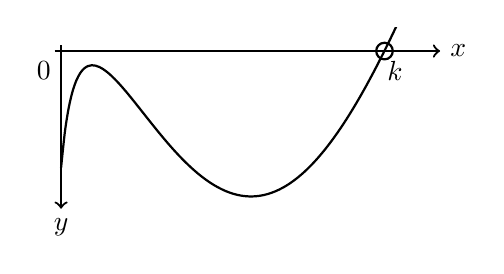
\begin{tikzpicture}
		\begin{axis}[thick,smooth,no markers , hide axis, height=4.4cm, width=8.0cm, ymin=-3.4, ymax=0.4, xmin=-1.0, xmax=7.0]
			\addplot+[black, samples=100, domain=0:6.0] {((15*x)/(1 + (3 * x))) - (2 + (5 * sin(((4 * pi * x)/(25)) r)))};
			\draw[arrows=->, thick] (axis cs:-0.1,0) -- (axis cs:6.0,0) node[right] {$x$};
			\draw[arrows=->, thick] (axis cs:0,0.1) -- (axis cs:0,-2.7) node[below] {$y$};
			\node[below left] at (axis cs:0, 0) {$0$};
			\node[below right] at (axis cs:5.0, 0) {$k$};
			\draw (axis cs:5.12, 0) circle (3pt);
		\end{axis} 
	\end{tikzpicture}
\end{center}
At point $k$, $A(t)$ intersects the x axis. Up until then, the amount of total sand has been decreasing (because $A(t)$ is below the x xis), and at $k$ it has been decreasing the longest. We can no integrate $A(t)$ from $0$ to $k$ to obtain the total amount of sand at that point:
\[ Y(k) \approx 2492.37 \enspace yd^3 \]


\pagebreak
\section{}
\subsection{Part A}
\pgfplotsset{ % Define a common style, so we don't repeat ourselves
	DiffEq/.style={
		width=0.6\textwidth, % Overall width of the plot
		axis equal image, % Unit vectors for both axes have the same length
		view={0}{90}, % We need to use "3D" plots, but we set the view so we look at them from straight up
		xmin=-1.7, xmax=1.7, % Axis limits
		ymin=-1.7, ymax=1.7,
		domain=-1:1, y domain=-1:1, % Domain over which to evaluate the functions
		hide axis,
		samples=3, % How many arrows?
		cycle list={    % Plot styles
			gray,
			quiver={
				u={1}, v={f(x)}, % End points of the arrows
				scale arrows=0.15,
				every arrow/.append style={
					-latex % Arrow tip
				},
			}\\
			red, samples=31, smooth, thick, no markers, domain=-1.1:1.1\\ % The plot style for the function
		}
	}
}

\begin{center}
	\begin{tikzpicture}[
		declare function={f(\x) = cos(pi * \x r)*(\y-1)^2;} % Define which function we're using
		]
		\begin{axis}[
			DiffEq, title={$\dfrac{dy}{dx}=(y-1)^2\cos{(\pi x)}$}
			]
			\addplot3 (x,y,0);
			\draw (axis cs:-1.4, 0.0) node[left] {$-1$} -- (axis cs:1.5, 0.0) node [right] {$1$};
			\draw (axis cs:0.0, -1.5) node[below] {$-1$} -- (axis cs:0.0, 1.4) node [above] {$1$};
		\end{axis}
	\end{tikzpicture}
\end{center}

\subsection{Part B}
Despite being able to simply look at the graph, we can infer that the slope from the differential equation will be zero at $y = 1$ because the entire equation is multiplied by $(y-1)^{-2}$.

\subsection{Part C}
\[ f(1) = 0; \enspace y = 0, \enspace x = 1 \]
\[ \frac{dy}{dx}=(y-1)^2\cos{(\pi x)} \]
\[ \frac{dy}{(y-1)^2}=\cos{(\pi x)}\,dx \]
\[ (y-1)^{-2}\,dy=\cos{(\pi x)}\,dx \]
\[ \int (y-1)^{-2}\,dy= \int \cos{(\pi x)}\,dx \]
\[ \frac{1}{1-0} = \frac{\sin{(\pi 1)}}{\pi} + C_3 \]
\[ 1 = 0 + C_3 \]
\[ 1 = C_3 \]
\[ \frac{1}{1-y} = \frac{\sin{(\pi x)}}{\pi} + 1 \]


\pagebreak
\section{}
\subsection{Part A}
\[ \int_{-1}^{10} (\sqrt{x - 1})\, dx \approx \]

\subsection{Part B}
\[ \pi\!\!\int_{-1}^{10} (x - 1)\, dx \approx \]

\subsection{Part C}
\[ y = \sqrt{x - 1} \]
\[ y^2 = x - 1 \]
\[ y^2 + 1 = x \]
\[ \pi\!\!\int_{0}^{3} (y^2 + 1)^2\,dy \approx \]


\pagebreak
\section{}
%\begin{center}
%	\begin{tikzpicture}
%		\begin{axis}[thick,smooth,no markers, hide axis, ymin=-3, ymax=2, xmin=-1, xmax=5]
%			\draw[thick, arrows=<-] (axis cs:0, 2) -- (axis cs:0, -3);
%			\draw[thick, arrows=->] (axis cs:-1, 0) -- (axis cs:5, 0);
%			\node[text, below left] at (axis cs:0.0, 0.0) {$O$};
%			\draw [cyan, samples=100] plot [smooth, tension=0.75] coordinates { (axis cs:-1,-3) (axis cs:0,-1) (axis cs:1,0) (axis cs:2,-1) (axis cs:3,-2) (axis cs:4,0) (axis cs:5,2) (axis cs:6,0) };
%		\end{axis}
%	\end{tikzpicture}
%\end{center}

\subsection{Part A}
1, 3, 5. This is because $f'(x)$ is zero (has a horizontal tangent) at these locations.

\subsection{Part B}
Min: $x = 4$, the graph had been negative until then, meaning that $f(x)$ decreased until this point. \\ \\
Max: $x = -1$, the graph stays negative for more of the graph between $-1 \leq x \leq 5$ than it stays positive. This means that there is no higher value of $f(x)$ than the beginning.

\subsection{Part C}
\[ g(x) = xf(x) \]
\[ g'(x) = (1)f(x) + xf'(x) \]
\[ m = g'(2) = (1)f(2) + xf'(2) = 6 + (2)(-1) = 6 - 2 = 4 \]
\[ y = f(2) = 6, \enspace x = 2 \]
\[ y - 6 = 4 (x - 2) \]


\pagebreak
\section{}
Not finished!

\pagebreak
\section{}
\[ h(x) = f(g(x))-6 \]
\[ h'(x) = f'(g(x))g'(x) \]
\begin{center}
	\begin{tabular}{ | c || c | c | c | c | c | c | }
		\hline
		\rule{0pt}{4ex}
		$x$ & $f(x)$ & $f'(x)$ & $g(x)$ & $g'(x)$ & $h(x)$ & $h'(x)$ \\
		\hline
		\hline
		1 & 6  & 4  & 2 & 5 & 3  & 2 \\
		\hline
		2 & 9  & 2  & 3 & 1 & 4  & -8 \\
		\hline
		3 & 10 & -4 & 4 & 2 & -7 & 21 \\
		\hline
		4 & -1 & 3  & 6 & 7 & & \\
		\hline
	\end{tabular}
\end{center}

\subsection{Part A}
$h(r)$ is continuous, $h(2) = 4$, and $h(3) = -7$. By \textit{IVT}, $\exists \enspace r \in [2, 3]$ such that $h(r) = -5$.

\subsection{Part B}
$h'(r)$ is continuous, $h(2) = -8$, and $h(3) = 21$. By \textit{IVT}, $\exists \enspace r \in [2, 3]$ such that $h'(r) = -5$.

\subsection{Part C}
\[ \int_{a}^{b} f(x) = F(b) - F(a) \]
\[ w(x) = \int_{1}^{g(x)} f(t)\,dt = F(1) - F(g(x)) \]
\[ w'(x) = f(1) - f(g(x))g'(x) \]
\[ w'(3) = f(1) - f(g(3))g'(3) = 6 - f(4)(2) = 6 + 2 = 8 \]

\subsection{Part D}
\[ y = g^{-1}(x), \enspace x = 2 \]
\[ y = g^{-1}(2), \enspace g(1) = 2, \enspace g^{-1}(2) = 1 \]
\[ m = g^{-1}'(2), \enspace g'(3) = 2, \enspace g^{-1}'(2) = 3 \]
\[ y - 1 = 3(x - 2) \]


\pagebreak
\section{}
\subsection{Part A}
\[ r - 30 = 2.0(t - 5) \]
\[ r - 30 = 2.0(5.4 - 5), \enspace r = 30.8 ft \]
\begin{center}
	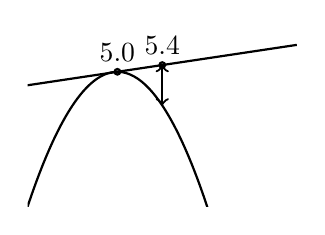
\begin{tikzpicture}
		\begin{axis}[thick,smooth,no markers, hide axis, xmin=-0.5, xmax=1.0, ymin=0.0, ymax=0.5, height=5cm, width=5cm]
			\addplot[samples=100, domain=-1.0:1.0] {-\x*\x + 0.25};
			\addplot[samples=100, domain=-1.0:1.0] {0.05*\x + 0.25};
			\draw[arrows=<->] (0.25, 0.2625) -- (0.25, 0.1875);
			\draw (axis cs:0.0, 0.25) circle(1pt) node[above] {$5.0$};
			\draw (axis cs:0.25, 0.2625) circle(1pt) node[above] {$5.4$};
		\end{axis} 
	\end{tikzpicture}
\end{center}
The approximation is above the actual value, because the line approximation will overshoot the decreasing (concave down) function.

\subsection{Part B}
\[ r(5) = 30, \enspace r'(5) = 2.0 \]
\[ \frac{dV}{dt} = \frac{d}{dt} \frac{4}{3}\pi r^3 = 4 \pi r^2 r' \]
\[ 4 \pi (30.0)^2(2.0) = 7200\pi \, ft^3/min \]

\subsection{Part C}
\[ \int_{0}^{12} r'(t)\,dt \approx \sum _{i=1}^{6}r'(t)_{i}\,\Delta t_{i} \approx \]
\[ (0.5)(1) + (0.6)(4) + (1.2)(2) + (2.0)(3) + (4.0)(2) = 19.3 \, ft\]
\underline{$\int_{0}^{12} r'(t)\,dt$} represents the number of feet the balloon has expanded (in radius) past it's original condition, and it is \textbf{not} the absolute radius of the balloon.

\subsection{Part D}
\begin{center}
	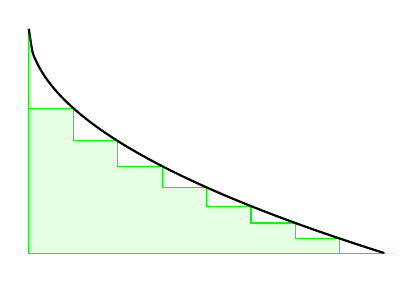
\begin{tikzpicture}
		\begin{axis}[
			height=5cm,
			width=7cm,
			xmin=0, xmax=1, ymin=0,ymax=1,
			hide axis,
			enlargelimits=true,
			clip=false,
			domain=0:1,
			axis on top
			]
			\addplot [draw=green, fill=green!10, const plot mark right, samples=9, domain=0:1] {1 - sqrt(\x)}\closedcycle;
			\addplot[smooth, thick,domain=0:1,samples=100]{1 - sqrt(\x)};
		\end{axis}
	\end{tikzpicture}
\end{center}

The RHS will under approximate the graph because it's slope is always negative, meaning any nonzero area under the curve from the right will undershoot it travelling left.


\end{document}
